% !TEX root = ../thesis.tex
\chapter{Návrh a implementácia riešenia zvolenej problematiky}\label{ch:design-implementation}

Pri tvorbe práce bol použitý prístup „comparative case study" založený na implementácii dvoch variantov rovnakého systému.

Použitá metodológia kombinuje prvky analytického a syntetického prístupu. Najskôr je systém rozdelený na jednotlivé architektonické aspekty, ktoré sú analyzované samostatne (komunikácia, perzistencia, transakcie, nasadenie). Následne sú tieto aspekty syntetizované do uceleného pohľadu na architektúru systému ako celku.

Takýto prístup umožňuje systematicky porovnať dva architektonické štýly bez toho, aby bol jeden z nich vopred preferovaný. Metodika je navrhnutá tak, aby bola reprodukovateľná a aby výsledky porovnania boli interpretovateľné aj v inom kontexte, než je konkrétny prototyp implementovaný v rámci tejto práce.

Metodika spočíva v:
\begin{itemize}
    \item definovaní jednotnej domény a rovnakých kľúčových use-caseov, ktoré sú implementované v oboch variantoch (monolit aj mikroservisy), aby bolo porovnanie férové a opakovateľné,
    \item implementácii monolitického prototypu s tradičnou vrstvenou štruktúrou a jednotnou databázou, kde je celý systém realizovaný ako jeden nasaditeľný celok (single deployable unit),
    \item implementácii mikroservisného prototypu s doménovým rozdelením služieb a event-driven koordináciou procesu, kde je riešenie rozdelené do samostatných služieb v rámci multi-modulového Maven projektu,
    \item systematickej dokumentácii architektúry, dátových tokov a technických rozhodnutí, pričom sa explicitne zaznamenávajú hranice domén (bounded contexts), spôsob komunikácie a dátové modely,
    \item príprave kritérií porovnania a návrhu experimentov zameraných na merateľné charakteristiky: zložitosť nasadenia, izolácia zlyhaní, konzistencia dát, rozsah potrebnej infraštruktúry, udržiavateľnosť a náročnosť zmien v doméne.
\end{itemize}

Dôležitým princípom je, že oba prototypy slúžia na porovnanie architektúr, preto je prístup k optimalizáciám pragmatický: prioritou je transparentnosť, reprodukovateľnosť a demonštrácia rozdielov, nie maximalizácia výkonu alebo úplná produkčná pripravenosť.

\section{Konceptuálny návrh riešenia}

Konceptuálny návrh vychádza z doménovej dekompozície rezervačného systému na štyri hlavné oblasti:
\begin{itemize}
    \item \textbf{Users} — správa používateľov a ich identifikácia,
    \item \textbf{Reservations} — evidencia rezervácií a ich životný cyklus,
    \item \textbf{Payments} — spracovanie platby a výsledku platby,
    \item \textbf{Notifications} — informovanie o výsledku (potvrdenie alebo zlyhanie).
\end{itemize}

V monolitickej verzii sú tieto oblasti realizované v rámci jedného systému ako logické moduly s priamou komunikáciou. V mikroservisnej verzii sú realizované ako autonómne služby.

Kľúčovým konceptuálnym rozdielom je transakčný model:
\begin{itemize}
    \item \textbf{Monolit} — jeden proces, jedna databáza, ACID transakcia pokrývajúca viac krokov.
    \item \textbf{Mikroservisy} — lokálne transakcie v každej službe, eventual consistency medzi službami, koordinácia cez udalosti~\cite{Vogels2009}.
\end{itemize}

Pre mikroservisnú verziu je rozhodujúce zavedenie event-driven koordinácie a spoľahlivej publikácie udalostí. Transactional outbox je v tomto kontexte kľúčový mechanizmus, ktorý zabezpečuje, že udalosť nebude „stratená" medzi commitom databázy a publikáciou do Kafka.

\section{Implementovaný prototyp}

Okrem čisto technického opisu komponentov je vhodné stručne opísať aj spôsob, akým sa prototyp používa z pohľadu scenára. V oboch verziách systém umožňuje vytvoriť rezerváciu a iniciovať spracovanie platby s následným prechodom rezervácie do výsledného stavu. Rozdiel je v tom, ako rýchlo je tento výsledok pozorovateľný a kde sa nachádza „hranica procesu": v monolite je proces typicky uzavretý v rámci jedného volania, v mikroservisoch je rozdelený do viacerých krokov spracovaných nezávisle.

Pri implementácii prototypu je dôležité poznamenať, že niektoré prvky boli zvolené ako pragmatické zjednodušenie pre účely porovnania. Typickým príkladom je správa schémy databázy automatickou aktualizáciou v monolite alebo zdieľaný modul so spoločnými definíciami v mikroservisoch. V produkčných systémoch by boli preferované explicitné migrácie a striktnejšie verzovanie kontraktov.

\subsection{Monolitická verzia}

Monolitická verzia je implementovaná ako jeden Spring Boot backend, ktorý je nasadzovaný ako jeden spustiteľný artefakt (jeden proces). V rámci jednej aplikácie sú implementované doménové časti pre používateľov, rezervácie, platby a notifikácie. Typickou charakteristikou monolitu je priama interná komunikácia medzi modulmi vo forme volania metód v rámci rovnakého runtime. Kľúčovým znakom je transakčné spracovanie: proces vytvorenia rezervácie a súvisiace kroky môžu byť realizované v rámci jednej databázovej transakcie, čo poskytuje silnú konzistenciu (ACID) v rámci jedného systému.

Monolit používa jednu databázu PostgreSQL (v prototypovej implementácii pomenovanú ako \texttt{reservation\_monolith\_db}) a perzistenciu realizuje pomocou Spring Data JPA. Cieľom monolitickej verzie v práci je slúžiť ako tradičný referenčný bod pre porovnanie s mikroservisnou verziou.

Architektúra monolitu:
\begin{itemize}
    \item jeden Spring Boot backend (jeden deployable artefakt),
    \item package-by-feature (users/reservations/payments/notifications),
    \item vrstvy controller/service/repository/entity v rámci jednotlivých domén.
\end{itemize}

Technológie:
\begin{itemize}
    \item Java 17, Spring Boot 3.2.3,
    \item Spring Data JPA, PostgreSQL,
    \item Maven ako build nástroj.
\end{itemize}

Perzistencia a transakcie:
\begin{itemize}
    \item jedna databáza \texttt{reservation\_monolith\_db},
    \item transakčné spracovanie v service vrstve cez \texttt{@Transactional}.
\end{itemize}

Na obrázku~\ref{fig:architecture-monolith} je zobrazená architektúra monolitickej verzie.

\begin{figure}[h]
    \centering
    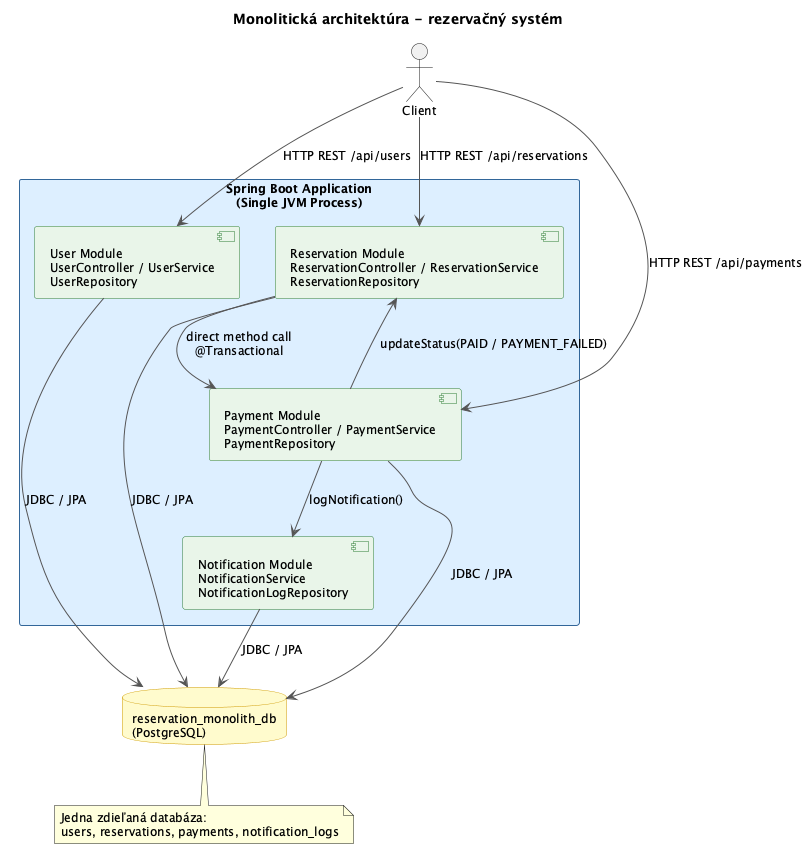
\includegraphics[width=0.85\textwidth]{figures/architecture-monolith.png}
    \caption{Architektúra monolitickej verzie}
    \label{fig:architecture-monolith}
\end{figure}

Na obrázku~\ref{fig:sequence-monolith} je zobrazený sekvenčný diagram toku vytvorenia rezervácie v monolite.

\begin{figure}[h]
    \centering
    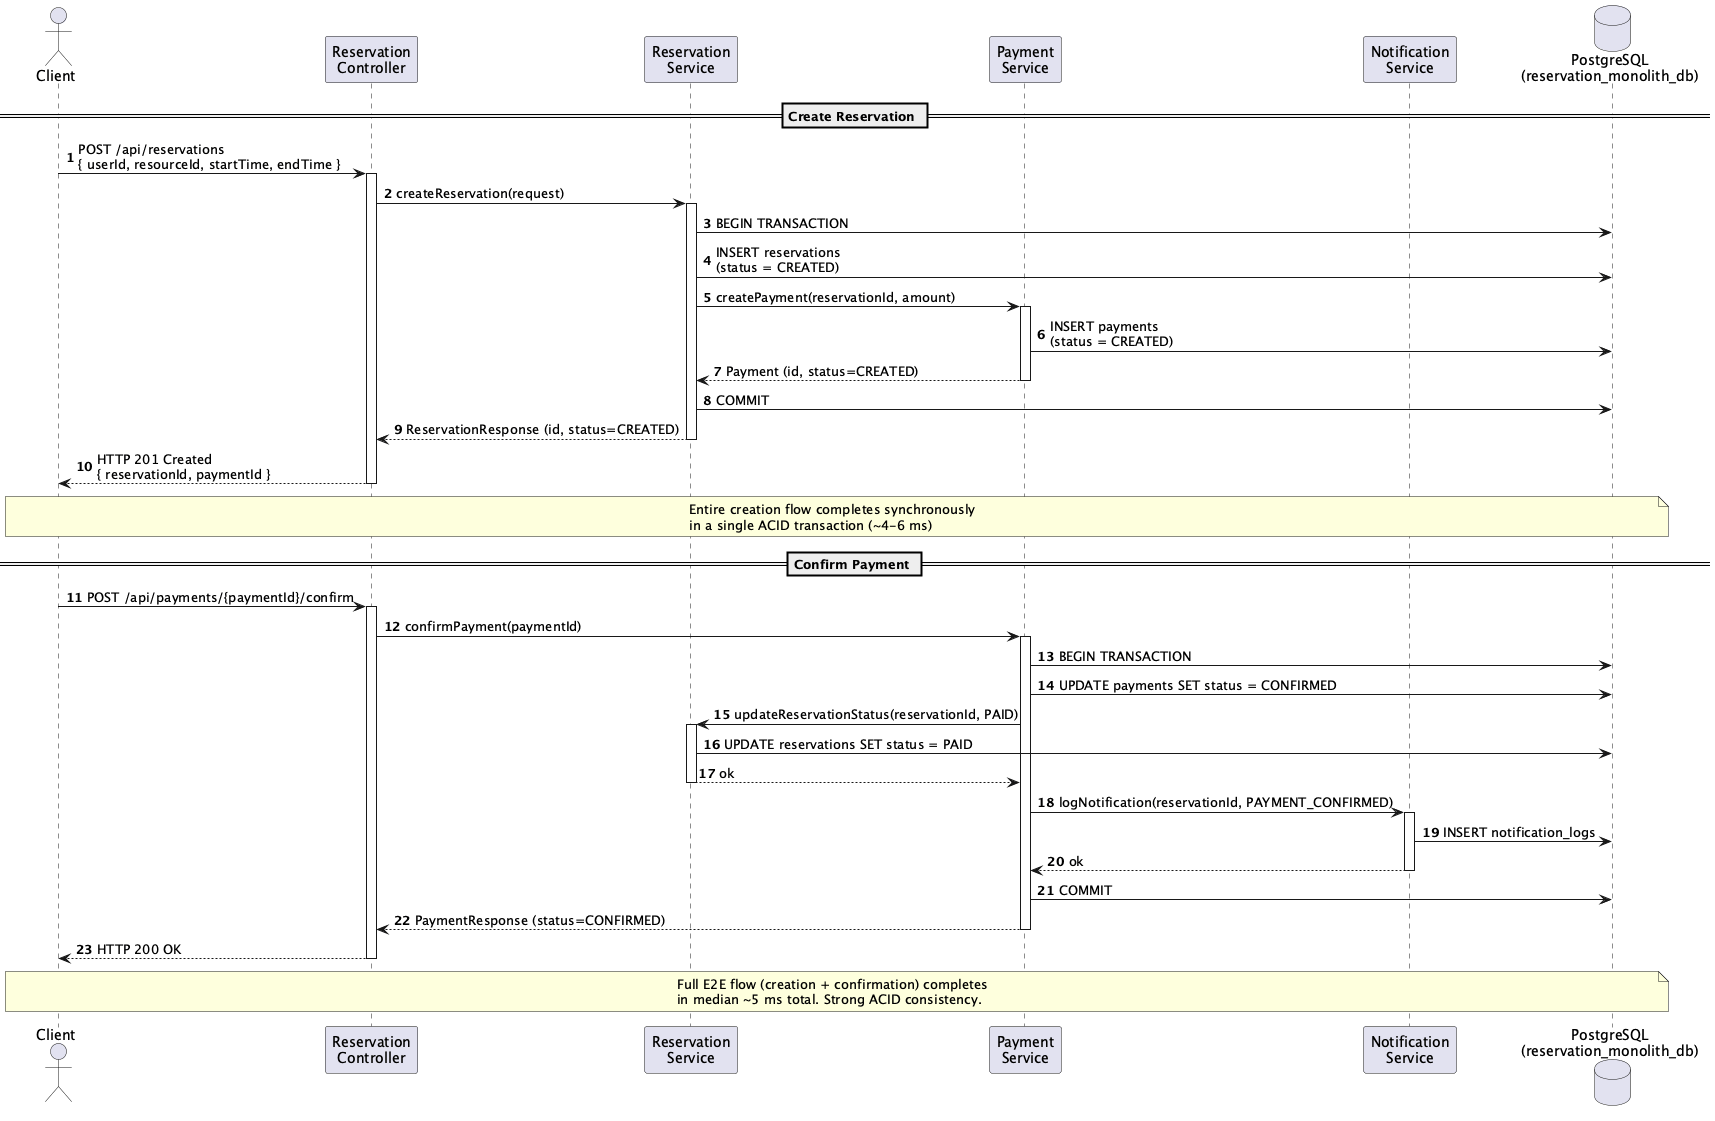
\includegraphics[width=0.85\textwidth]{figures/sequence-monolith.png}
    \caption{Sekvenčný diagram -- monolitická verzia}
    \label{fig:sequence-monolith}
\end{figure}

\subsection{Mikroservisná verzia}

Mikroservisná verzia je navrhnutá ako súbor samostatných služieb (mikroservisov), ktoré reprezentujú jednotlivé doménové oblasti:
\begin{itemize}
    \item \textbf{gateway-service} — centrálny vstupný bod (API Gateway),
    \item \textbf{user-service} — správa používateľov,
    \item \textbf{reservation-service} — spracovanie rezervácií,
    \item \textbf{payment-service} — spracovanie platieb,
    \item \textbf{notification-service} — notifikácie,
    \item \textbf{common} modul — zdieľaný „shared kernel" pre spoločné definície udalostí/DTO v rámci prototypu.
\end{itemize}

Služby sú implementované v Java 17 a Spring Boot 3.4.0. Externá komunikácia klienta prebieha synchrónne cez API Gateway, pričom vnútorný proces spracovania rezervácie je realizovaný asynchrónne cez Apache Kafka. Mikroservisná verzia je preto orientovaná na event-driven architektúru a demonštruje choreografiu sagy: jednotlivé služby reagujú na udalosti a posúvajú proces dopredu bez centrálneho koordinátora.

Dátová perzistencia je riešená princípom „database-per-service" na úrovni logických databáz v rámci jedného PostgreSQL servera (t.\,j. každá služba používa vlastnú databázu, napr. \texttt{user\_db}, \texttt{reservation\_db}, \texttt{payment\_db}, \texttt{notification\_db}). Pre zabezpečenie spoľahlivej publikácie udalostí je použitý mechanizmus transactional outbox v službách reservation-service a payment-service~\cite{Richardson2018}.

\begin{lstlisting}[language=Java, caption={Transactional Outbox -- atomické uloženie udalosti v rámci jednej transakcie (PaymentService.java)}]
@Transactional
public PaymentResponse confirm(Long id) {
    Payment payment = getPayment(id);
    payment.setStatus(PaymentStatus.CONFIRMED);

    PaymentConfirmedEvent event = new PaymentConfirmedEvent(
            payment.getId(), payment.getReservationId(),
            toEventStatus(payment.getStatus())
    );

    // Udalosť sa ukladá do outbox tabuľky v TEJ ISTEJ transakcii
    OutboxEvent outboxEvent = OutboxEvent.builder()
            .aggregateType("Payment")
            .aggregateId(payment.getId())
            .eventType(event.getClass().getName())
            .payload(objectMapper.writeValueAsString(event))
            .status(OutboxEventStatus.NEW)
            .createdAt(LocalDateTime.now())
            .build();
    outboxEventRepository.save(outboxEvent);

    return toResponse(payment);  // commit = atomova operacia
}
\end{lstlisting}

\begin{lstlisting}[language=Java, caption={Outbox scheduler -- polling a publikácia udalostí do Kafka (OutboxEventPublisher.java)}]
@Scheduled(fixedDelayString = "${app.outbox.scheduler-fixed-rate}")
@Transactional
public void publishOutboxEvents() {
    List<OutboxEvent> newEvents =
            outboxEventRepository.findByStatus(OutboxEventStatus.NEW);

    for (OutboxEvent event : newEvents) {
        try {
            Object kafkaEvent = objectMapper.readValue(
                    event.getPayload(), Class.forName(event.getEventType()));
            if (kafkaEvent instanceof PaymentConfirmedEvent confirmed) {
                paymentProducer.sendPaymentConfirmedEvent(confirmed)
                        .get(5, TimeUnit.SECONDS);
            } else if (kafkaEvent instanceof PaymentFailedEvent failed) {
                paymentProducer.sendPaymentFailedEvent(failed)
                        .get(5, TimeUnit.SECONDS);
            }
            event.setStatus(OutboxEventStatus.SENT);
        } catch (Exception e) {
            event.setStatus(OutboxEventStatus.FAILED);
        }
    }
    outboxEventRepository.saveAll(newEvents);
}
\end{lstlisting}

Architektúra mikroservisov:
\begin{itemize}
    \item gateway-service ako centrálna brána,
    \item user-service, reservation-service, payment-service, notification-service ako doménové služby,
    \item common modul pre zdieľané definície udalostí/DTO v rámci prototypu,
    \item hlavný proces rezervácie realizovaný event-driven cez Kafka.
\end{itemize}

Technológie:
\begin{itemize}
    \item Java 17, Spring Boot 3.4.0, Spring Cloud (Gateway),
    \item Apache Kafka (Spring Kafka),
    \item PostgreSQL (oddelené databázy na úrovni logických DB),
    \item Docker Compose pre lokálne spustenie~\cite{DockerCompose2025}.
\end{itemize}

Konzistencia a spoľahlivosť:
\begin{itemize}
    \item transactional outbox v reservation-service a payment-service,
    \item DLT pre spracovanie chýb v Kafka konzumácii,
    \item Actuator endpoints (health/info) pre základnú diagnostiku.
\end{itemize}

Na obrázku~\ref{fig:components} je zobrazená komponentová architektúra mikroservisnej verzie.

\begin{figure}[h]
    \centering
    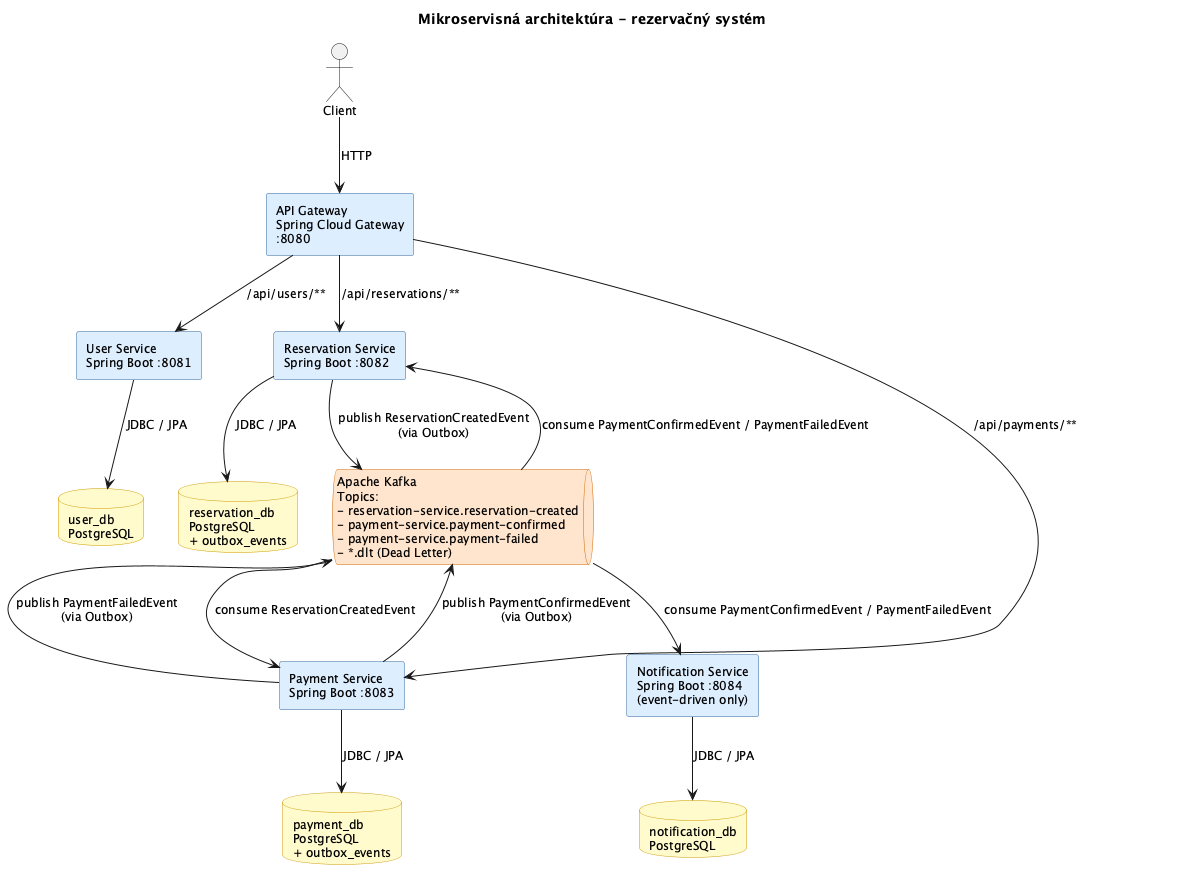
\includegraphics[width=0.9\textwidth]{figures/components.png}
    \caption{Komponentová architektúra mikroservisnej verzie}
    \label{fig:components}
\end{figure}

Na obrázku~\ref{fig:sequence-micro} je zobrazený sekvenčný diagram toku vytvorenia rezervácie v mikroservisnej verzii.

\begin{figure}[h]
    \centering
    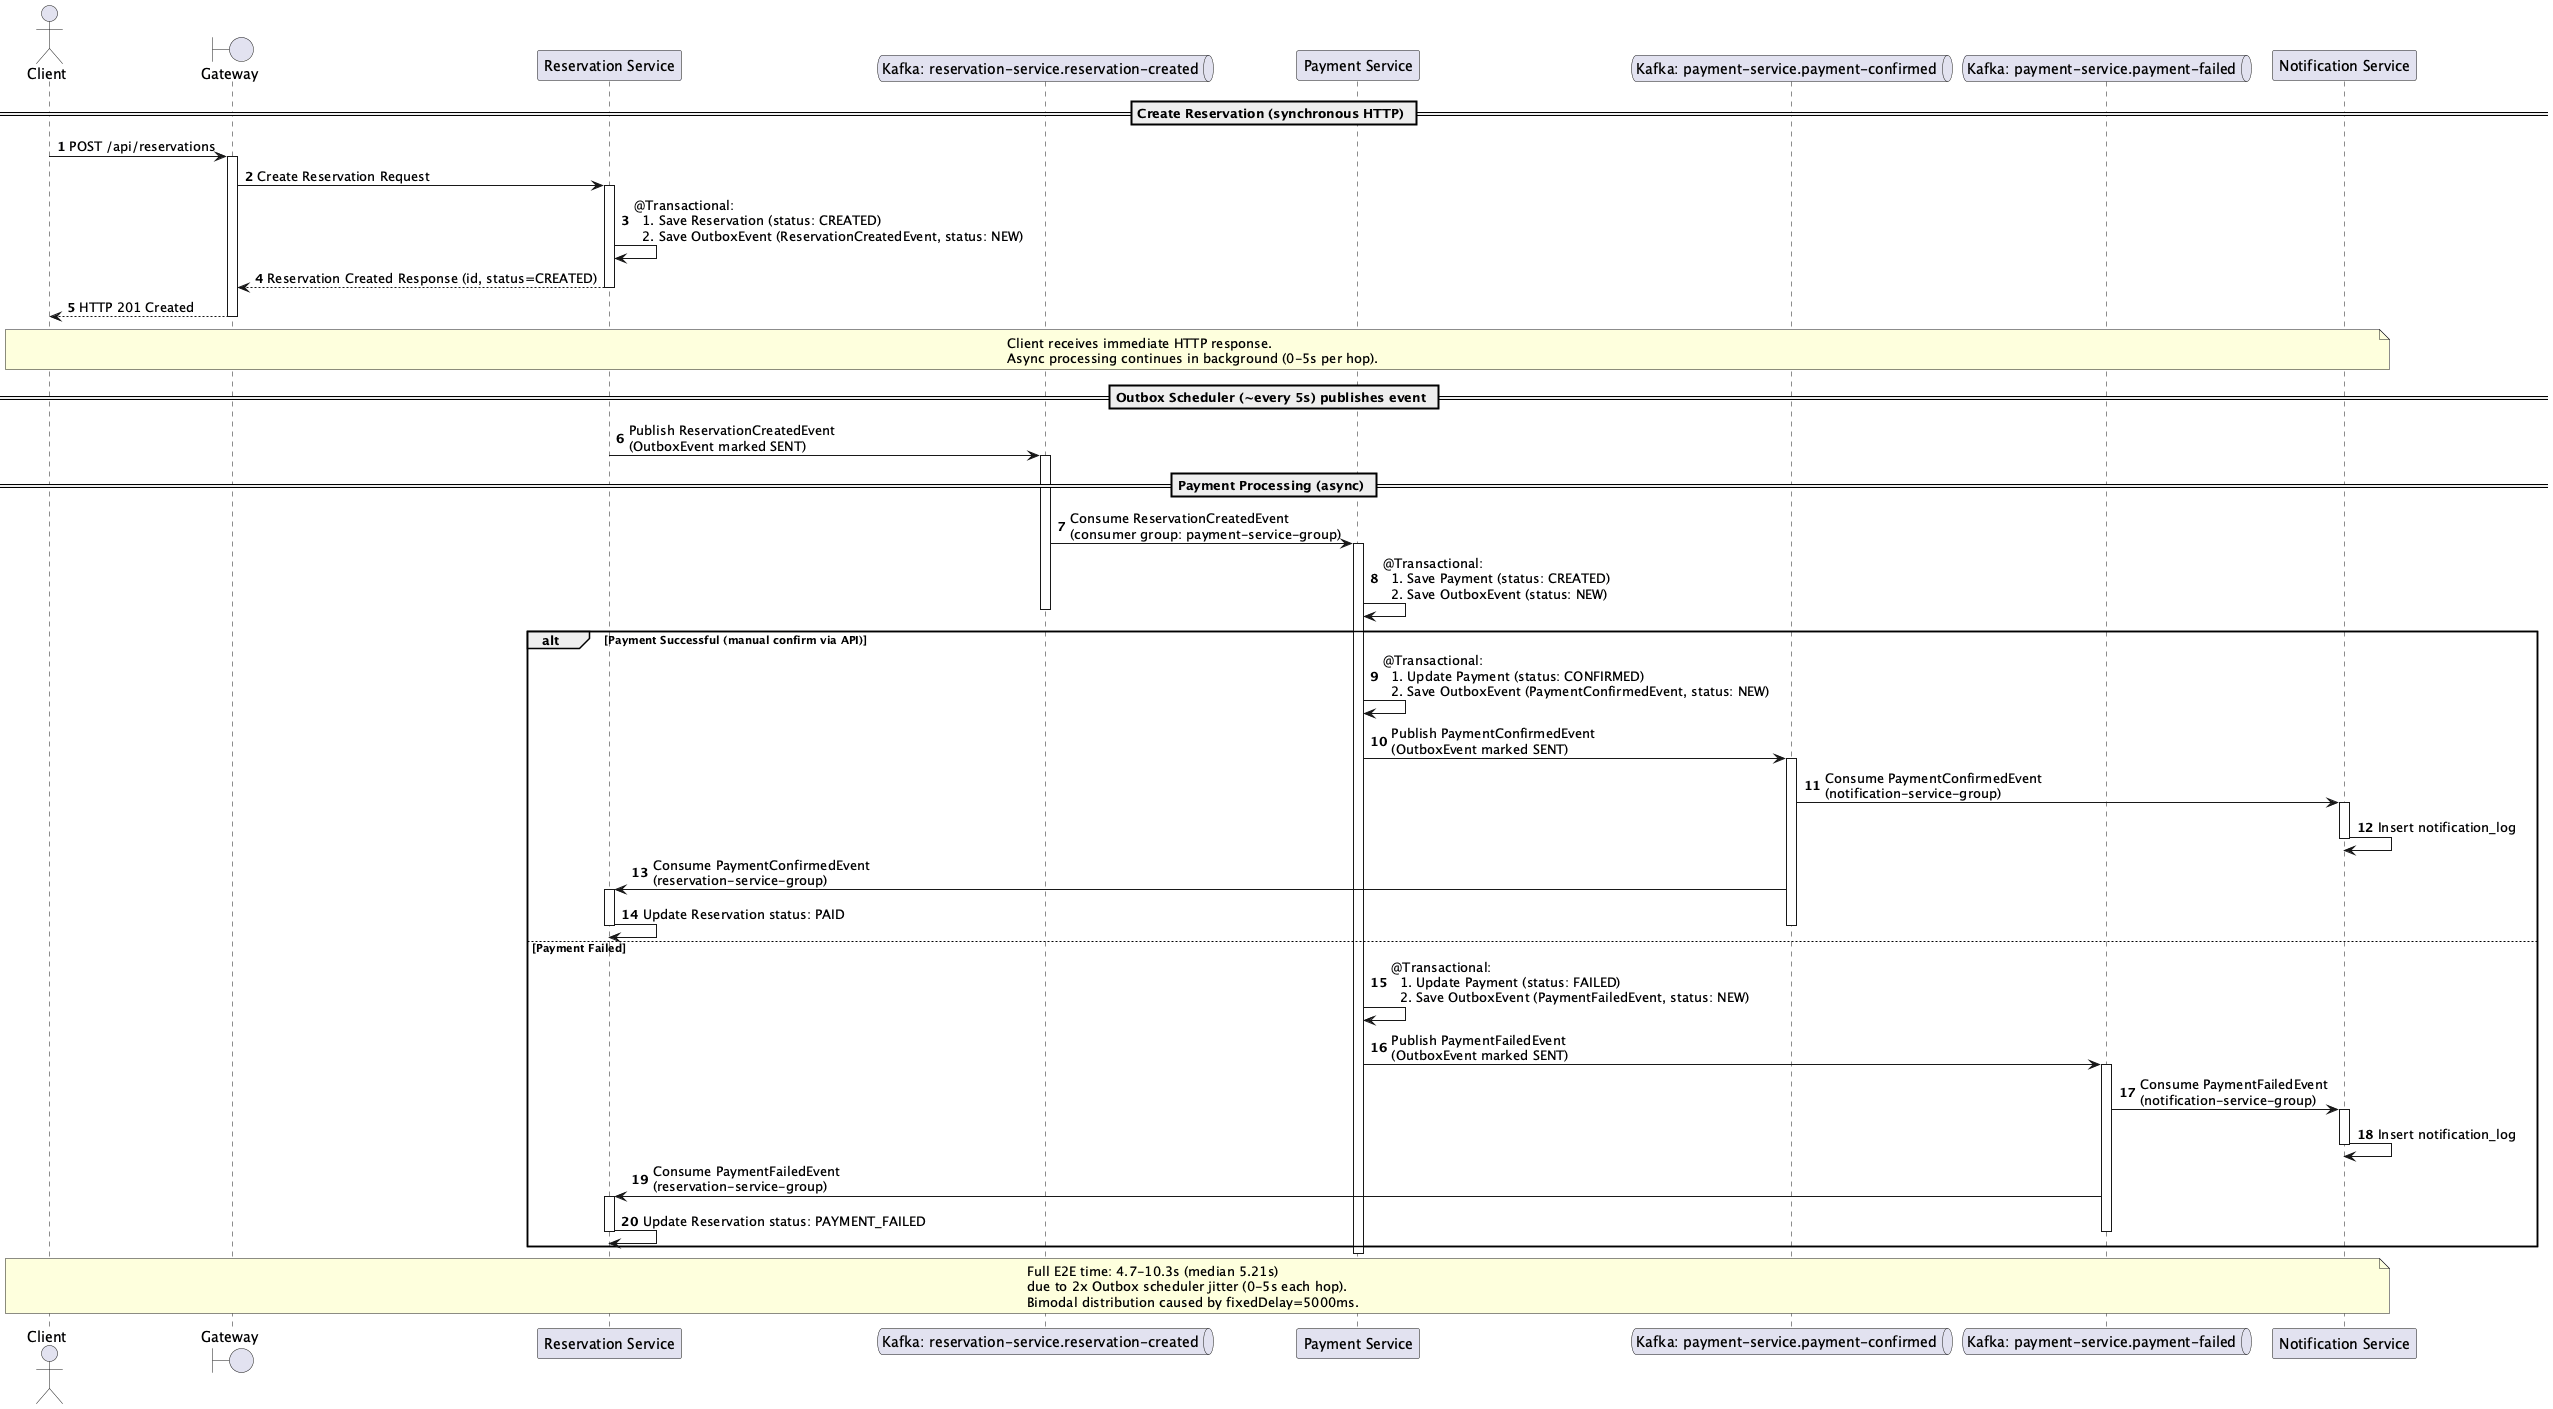
\includegraphics[width=0.9\textwidth]{figures/sequence.png}
    \caption{Sekvenčný diagram -- mikroservisná verzia}
    \label{fig:sequence-micro}
\end{figure}

ERD diagramy jednotlivých domén sú zobrazené na obrázkoch~\ref{fig:erd-reservation} a~\ref{fig:erd-payment}.

\begin{figure}[h]
    \centering
    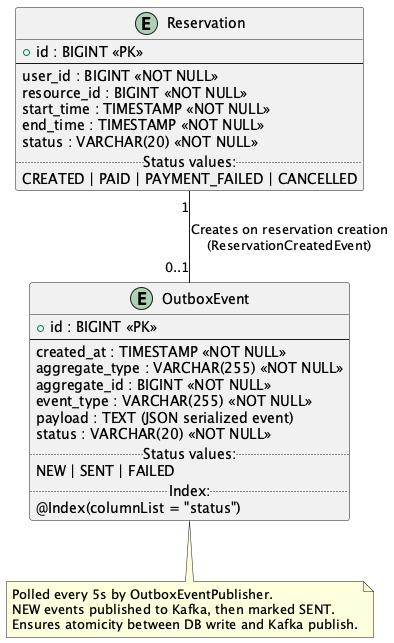
\includegraphics[width=0.75\textwidth]{figures/erd-reservation.png}
    \caption{ERD -- reservation-service}
    \label{fig:erd-reservation}
\end{figure}

\begin{figure}[h]
    \centering
    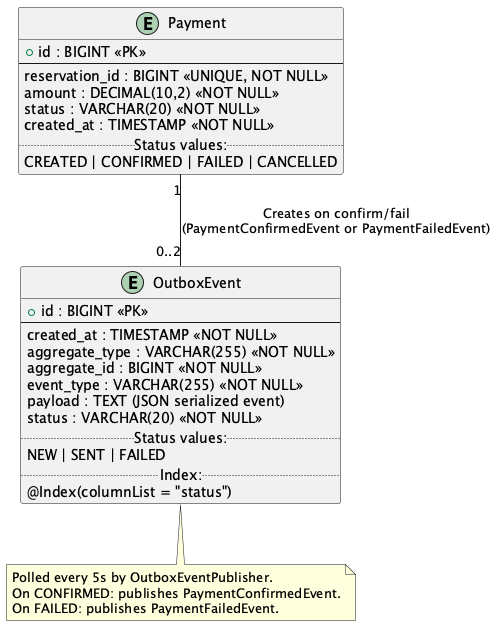
\includegraphics[width=0.75\textwidth]{figures/erd-payment.png}
    \caption{ERD -- payment-service}
    \label{fig:erd-payment}
\end{figure}

\subsection{Funkčná ekvivalencia}

Funkčná ekvivalencia v tejto práci znamená, že oba prototypy podporujú rovnaké kľúčové doménové operácie a vedú k rovnakým výsledným stavom procesu.

V oboch verziách je možné:
\begin{itemize}
    \item spravovať používateľov (základné operácie nad používateľskou entitou),
    \item vytvoriť rezerváciu,
    \item spracovať platbu asociovanú s rezerváciou,
    \item vyvolať notifikačný krok po potvrdení alebo zlyhaní platby.
\end{itemize}

Rozdiel medzi verziami spočíva v tom, ako je tento proces implementovaný (jedna transakcia a priame volania v monolite vs.\ asynchrónna choreografia cez udalosti v mikroservisnej verzii), nie v samotnom cieľovom správaní systému.

\subsection{Dátový model a API kontrakty}

Pri návrhu API kontraktov je dôležité dbať na stabilitu rozhraní a jasnú zodpovednosť za dáta. V monolitickej architektúre sú interné hranice často implicitné — jednotlivé moduly môžu zdieľať entity alebo priamo volať služby. Naopak, v mikroservisnej architektúre sa hranice materializujú ako verejné rozhrania (HTTP API alebo event kontrakty), ktoré by mali byť navrhnuté tak, aby minimalizovali potrebu častých zmien.

Z pohľadu dátového modelu je rozdiel medzi „zdieľanou schémou" a „rozdelenou perzistenciou" kľúčový. Monolit môže používať jednotné referenčné väzby (napr. cudzie kľúče) naprieč doménami, čo uľahčuje dotazy a reportovanie. Mikroservisná architektúra naopak uprednostňuje vlastné dátové modely v rámci každej služby a komunikáciu cez správy alebo API. To znižuje prepojenosť, ale môže viesť k potrebe redundancie údajov.

Z pohľadu prototypu je dôležité zdokumentovať minimálne tieto kontrakty:
\begin{itemize}
    \item vstupné HTTP rozhranie pre vytvorenie rezervácie (volané cez gateway, smerované do reservation-service),
    \item udalosti publikované do Kafka, najmä \texttt{ReservationCreated} a \texttt{PaymentConfirmed/PaymentFailed},
    \item spôsob zmeny stavu rezervácie v reakcii na výsledok platby.
\end{itemize}

\subsection{Spustenie a testovanie}

Reprodukovateľné spustenie predstavuje dôležitý predpoklad pre korektné porovnanie. V monolitickej verzii typicky postačuje spustenie jednej aplikácie a jednej databázy. V mikroservisnom variante však lokálne prostredie simuluje distribuovaný systém: okrem databáz je potrebný message broker a viacero bežiacich služieb. Docker Compose v tomto kontexte poskytuje praktický spôsob, ako definovať infraštruktúru deklaratívne a spúšťať ju konzistentne~\cite{DockerCompose2025}.

Mikroservisná verzia je spustiteľná v lokálnom prostredí pomocou Docker Compose, ktorý definuje závislosti na Kafka/Zookeeper a PostgreSQL, a zároveň spúšťa jednotlivé služby v kontajneroch. Použitý je koncept Spring Profiles, kde sa odlišuje základná konfigurácia a konfigurácia určená pre docker prostredie (\texttt{application.yml} a \texttt{application-docker.yml}).

Na úrovni testovania je v prototypoch prítomná podpora jednotkových a integračných testov (závislosti na JUnit 5, Mockito a súvisiace testovacie nástroje). Mikroservisná verzia zároveň využíva Actuator a exponuje základné health/info endpointy.

